\section{One Time Password}
\label{arquitectura:otp}
%\textbf{Oscar}: \textit{Posa com el generes, com es valida, validesa + més flux de comunicació amb l'usuari}
L'últim ``subsistema'' dins del \textit{backend} a tenir en compte, és el de la generació de codis OTP.\\
Aquest respon a la necessitat de disposar d'un mètode de signatura per als consentiments informats que es generen.\\
\newline Per tant, amb aquesta premissa podem identificar casos d'ús que es mostren a la figura:
\begin{figure}[h]
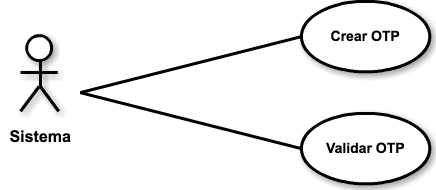
\includegraphics[scale=0.4]{sections/arquitectura/otp_useCase.png}
\centering
\caption{OTP - Casos d'ús}
\label{fig:otp_workflow}
\end{figure}
\begin{itemize}
    \item Crear OTP\\
    En el moment de la signatura electrònica,el sistema ha de ser capaç de generar un codi numèric basat en l'instant de temps del sistema (\textit{Unix time}) i una clau secreta de cada usuari.
    Un cop generat, aquest codi s'enviarà a l'usuari.
    \item Validar OTP\\
    El sistema ha de ser capaç, donat un codi OTP i una clau, de determinar si l'OTP donat és vàl·lid o no.
\end{itemize}
La imatge següent il·lustra el funcionament de cadascún dels casos d'ús de forma separada.
\begin{figure}[h]
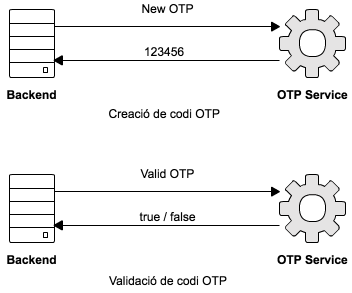
\includegraphics[scale=0.5]{sections/arquitectura/otp_architecture_useCase.png}
\centering
\caption{OTP - Arquitectura del sistema}
\label{fig:otp_workflow}
\end{figure}
\newline Tot i tractar-se de funcionalitats diferents, ambdues queden incloses dins del mateix servei.\\
\newline La clau secreta dels usuaris es troba emmagatzemada a la base de dades del sistema. Tot i això, el servei no accedeix a la base de dades.\\
En aquest cas, a diferència dels sistemes anteriors, no es requereix de serveis externs per a dur a terme les tasques que s'esperen del servei.

%En el context d'aquest projecte, la validació de la identitat de l'usuari serveix per a iniciar el procés de signatura del consentiment informat generat prèviament per l'ocasió.\\
%Per a signar el document, com s'ha esmentat prèviament, es fa ús de codis OPT generats al moment i enviats a l'usuari via el servei de missatgeria. %\textit{Clickatell}\footnote{https://www.clickatell.com/}.\\
%\newline A continuació es pot veure (Figura \ref{fig:otp_workflow}) el flux d'execució que segueix la plataforma:
%\begin{figure}[h]
%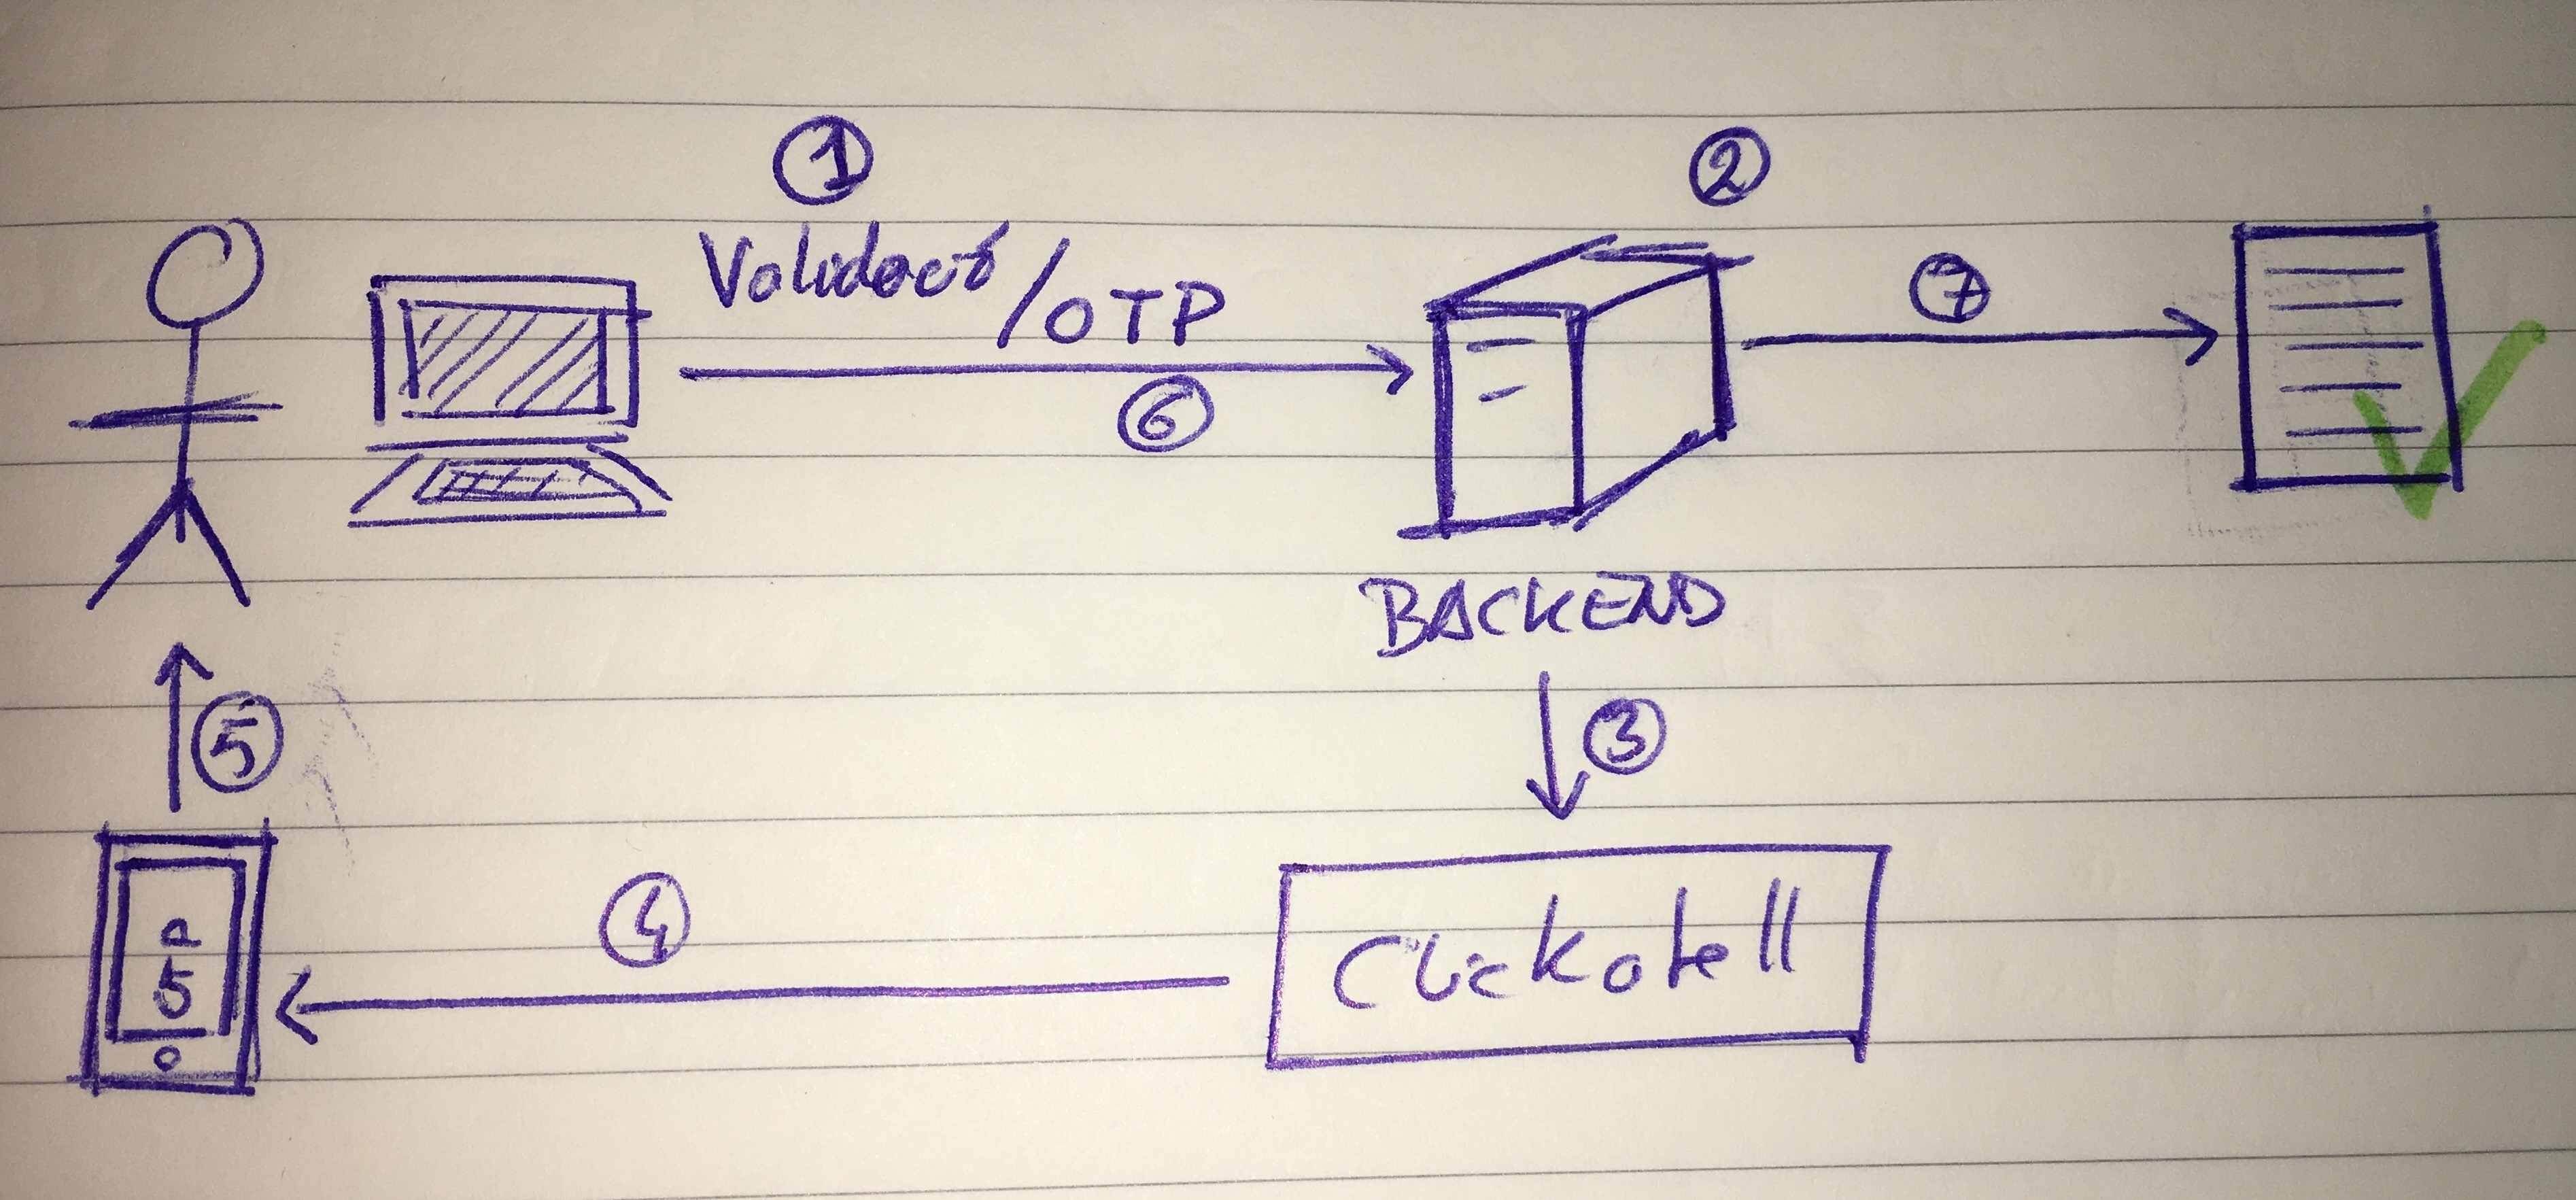
\includegraphics[scale=0.1]{sections/arquitectura/otp_workflow.jpg}
%\centering
%\caption{Fluxe d'events del codi OTP}
%\label{fig:otp_workflow}
%\end{figure}
%\newline Els diferents punts de la figura fan referència als diferents passos del procés de signatura:
%\begin{enumerate}
%    \item L'usuari valida la seva identitat mitjançant la introducció de la contrassenya de la plataforma.
%    \item El \textit{backend} comprova la identitat. En cas afirmatiu genera el codi OTP. En cas contrari, mostra el missatge pertinent.
%    \item S'envia el codi OTP a \textit{Clickatell} a través de la API del servei.
%    \item \textit{Clickatell} envia via SMS el codi OTP.
%    \item L'usuari rep el codi SMS i l'introdueix a la plataforma.
%    \item El sistema valida el codi OTP.
%    \item El document queda signat.
%\end{enumerate}
%\newline Amb una mica mes de detall, l'usuari rep de la mà de \textit{CLickatell} un SMS com el que es mostra a la Figura \ref{fig:arquitectura_otp}:
%\begin{figure}[h]
%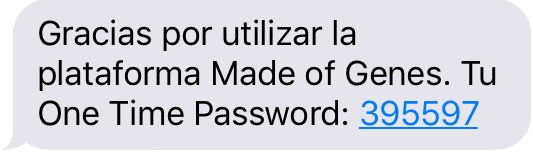
\includegraphics[scale=0.3]{sections/arquitectura/sms_otp.jpg}
%\centering
%\caption{SMS amb codi OTP}
%\label{fig:arquitectura_otp}
%\end{figure}
%\newline La generació del codi, es fa amb l'algorisme especificat a l'RFC6238\footnote{https://tools.ietf.org/html/rfc6238}.\\
%Aquest algorisme ha estat encapsulat en un servei independent per tal d'oferir funcions de generació així com de validació de codis OTP.\\
%\newline Per a generar els codis OTP, el servei fa ús del \textit{Unix timestamp} i una clau alfanumèrica secreta generada automàticament per cada usuari.\\
%Un cop generat el codi, s'envia a l'usuari a través d'un SMS.\\
%\newline Rebut el codi, l'usuari disposa aproximadament de tres minuts per introduir-lo al camp de text pertinent al \textit{frontend} de la plataforma, tal i com es pot apreciar a la figura següent: 
%\begin{figure}[h]
%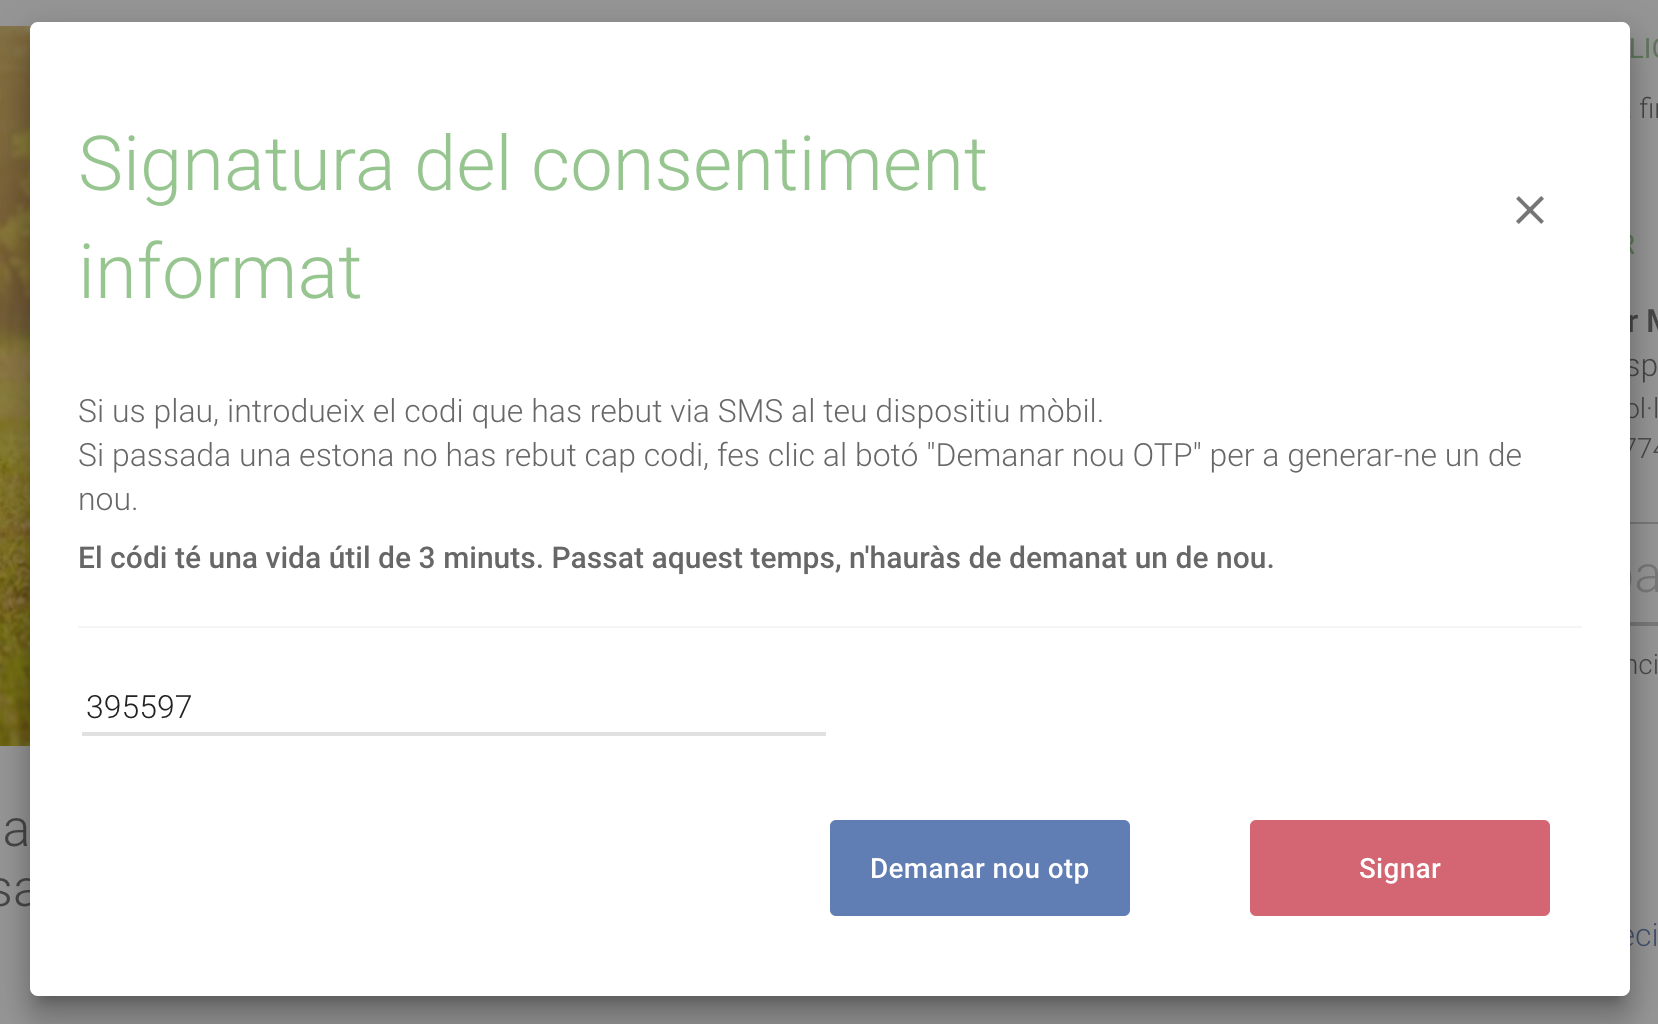
\includegraphics[scale=0.3]{sections/arquitectura/frontend_otp.png}
%\centering
%\caption{Signatura del consentiment informat amb el codi OTP}
%\label{fig:arquitectura_otp_frontend}
%\end{figure}
%A l'hora de validar el codi, el sistema genera altre cop un codi OTP i el compara amb el que rep per part de l'usuari. Això és possible gràcies a la finestra de temps que fa servir l'algorisme a l'hora de generar l'OTP.\\
%\newline Per entendre'ns, un cop obtingut el \textit{Unix timestamp} del sistema, s'aplica sobre aquest el que s'anomena finestra de temps (definida com a constant al codi) i n'obté un valor a partir del qual es calcularà el codi. Aquest valor, no canviarà fins que no se superi un temps determinat.\\
%Per tant, donada una clau d'usuari, si no s'ha superat el temps de validesa del codi OTP de l'usuari, el sistema és capaç de generar-ne un d'igual, i així comprovar-ne la validesa.\\
%\newline Un cop validat el codi entrat per l'usuari, el sistema llança el procés que certifica la signatura del consentiment informat.


%La contrasenya d’un sol ús, altrament anomenada \textit{One Time Password}, en endavant OTP, és una contrasenya que tal i com indica el seu nom, és vàl·lida per una sola vegada. Un cop emprada, se n’ha de generar una de nova o bé demanar al proveïdor pertinent que en faciliti una de nova;en qualsevol dels casos un cop feta servir, se n’ha d’adquirir una de nova.\\
%\newline Aquest tipus de pràctica apareix a partir de les cada cop més evidents mancances de la contrasenya estàtica original, que es veuen accentuades amb l’imparable creixement que d’internet.\\
%\newline L’ús principal dels OTP es troba en el que s’anomena autenticació en 2 passos, un procés que busca assegurar la identitat de l’usuari mitjançant un segon pas en el procés convencional d’autenticació clàssic a partir de nom d’usuari i contrasenya, consistent en la introducció d’un codi que només l’usuari que s’autentica coneix.\\
%\newline La implementació que se'n fa dins del projecte es basa en aquella especificada a l'RFC6238, que porta per títol \textit{TOTP: Time-Based One-Time Password Algorithm}.\\
%\newline L'anterior document descriu una extensió de l'algorisme de OTP,descrit a l'RFC4226, amb títol \textit{HOTP: An HMAC-Based One-Time Password Algorithm}